\documentclass{beamer}
\usepackage{listings}
\lstset{
%language=C,
frame=single, 
breaklines=true,
columns=fullflexible
}
\usepackage{subcaption}
\usepackage{url}
\usepackage{amsmath}

\usepackage{amsthm}

\usepackage{tikz}
\usepackage{graphicx}
\usepackage{tkz-euclide} % loads  TikZ and tkz-base
%\usetkzobj{all}
\usetikzlibrary{calc,math}
\usepackage{float}

\newcommand\norm[1]{\left\lVert#1\right\rVert}
\renewcommand{\vec}[1]{\mathbf{#1}}
\newcommand{\R}{\mathbb{R}}
\newcommand{\C}{\mathbb{C}}
\providecommand{\brak}[1]{\ensuremath{\left(#1\right)}}
\providecommand{\abs}[1]{\vert#1\vert}
\providecommand{\fourier}{\overset{\mathcal{F}}{ \rightleftharpoons}}
\newcommand{\myvec}[1]{\ensuremath{\begin{pmatrix}#1\end{pmatrix}}}
\providecommand{\mean}[1]{E[ #1 ]}
\providecommand{\sbrak}[1]{\ensuremath{{}\left[#1\right]}}
\providecommand{\cbrak}[1]{\ensuremath{\left\{#1\right\}}}

\newcounter{saveenumi}
\newcommand{\seti}{\setcounter{saveenumi}{\value{enumi}}}
\newcommand{\conti}{\setcounter{enumi}{\value{saveenumi}}}

\usepackage[export]{adjustbox}
\usepackage[utf8]{inputenc}
\usepackage{amsmath}
\usetheme{Boadilla}
\title{Enhanced Secure Wireless Information and Power Transfer via Intelligent Reflecting Surface}
\author{Gaureesh K}
\date{EP20BTECH11005}
\begin{document}

\begin{frame}
\titlepage
\end{frame}
\begin{frame}{Aim}
    The aim of this paper is to devise an intelligent reflecting surface(IRS) aided
    secure wireless information and power transfer and maximise the harvested power.
    
\end{frame}

\begin{frame}{Abstract}
\begin{enumerate}
    \item Optimize the secure transmit beamforming
at the access point (AP) and phase shifts at the IRS subject to
the secrecy rate (SR) and the reflecting phase shifts at the IRS
constraints
    \item convert the optimization
problem into a semidefinite relaxation (SDR) problem and a
sub-optimal solution is obtained.
    \item To reduce the high-complexity
of the proposed SDR method, a low-complexity alternating
optimization (LC-AO) algorithm is proposed.
    \item  Simulation results
show that the harvested power of the proposed SDR and LC-AO
methods approximately double that of the existing method
without IRS with the same SR.
\end{enumerate}

\end{frame}

\begin{frame}{Introduction}
\begin{enumerate}
    \item There have been some innovative studies on the IRS-assisted wireless communication systems by jointly optimizing the beamforming vector and the phase shifts at the IRS.
    
    \item In a single-user multiple-input single-output
(MISO) scenario [5], semidefinite relaxation (SDR) and
Gaussian randomization algorithms were proposed to obtain
a sub-optimal solution to maximize the total received signal
power.
    
    \item simultaneous wireless information and
power transfer (SWIPT) could enhance the energy efficiency
and solve energy-limited issues of wireless networks to some
extent.
    \item However, due to the severe path loss, wireless power
transfer was only suitable for short distance transmission,
hence the range of energy harvesting receivers (EHR) is limited.
\end{enumerate}
\end{frame}

\begin{frame}{System Model}
    \begin{figure}[htp]
    \centering
    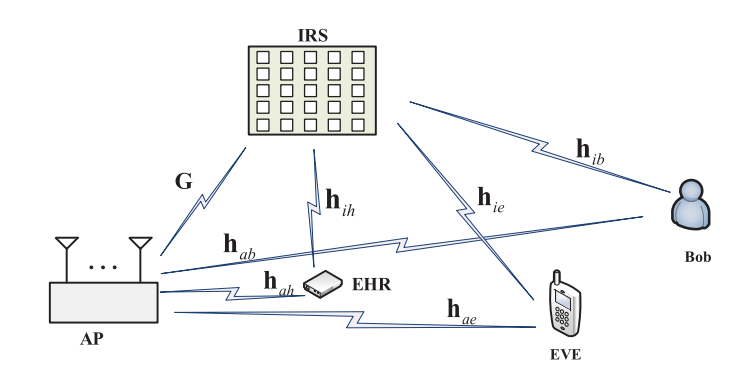
\includegraphics[width=10cm]{fig1.png}
    \caption{Fig. 1. An IRS-aided secure SWIPT wireless network.}
    \label{Fig. 1.}
\end{figure}
\end{frame}

\begin{frame}{System Model Contd.} 
Fig. 1 sketches a downlink MISO system with an IRS
for SWIPT.In Fig. 1, there are an AP with M transmit
antennas, an IRS with N reflecting units, an information receiver denoted as Bob, and an EHR in the presence of an EVE(eavesdropper).The minimum requirement for EHR such as the low-power
sensors is -10 dBm, which is much higher than that for Bob
(-60 dBm). Therefore, EHR should be placed close to the
AP. Besides, as shown in Fig. 1, an IRS is deployed in the
vicinity of EHR. The transmit signal from AP
can be expressed as
\begin{align}
    \textbf{x}=\textbf{w}s
\end{align}
where w $\in$ $\mathbb{C}^{M \times 1}$ denotes the transmit beamforming vector,
which forces the confidential message (s) to the desired direction.
\end{frame}

\begin{frame}{System Model Contd.}
 Suppose that $P_{s}$ is the total transmission power constraint. Thus,
we have $\mathbb{E}(x^{H}x)=\norm{\textbf{w}}^2\leq P_{s}$.
Let the baseband equivalent channel responses from the AP to the
IRS, from the AP to Bob, from the AP to EHR, from the AP to
EVE, from the IRS to Bob, from the IRS to the EHR, from the
IRS to EVE are denoted by G $\in$ $\mathbb{C}^{N\times M}$ , $h^{H}_{ab}$
 $\in$ $C^{1\times M}$ , $h^{H}_{ah}$ \in$
$C^{1\times M}$$, $h^{H}_{ae}$
 $\in$ $\mathbb{C}^{1\times M}$, $h^{H}_{ib}$
 $\in$ $\mathbb{C}^{1 \times N}$ , $h^{H}_{ih}$
 $\in$ $\mathbb{C}^{1 \times N}$ , $h^{H}_{ie}$
 $\in$ $\mathbb{C}^{1 \times N}$ , respectively. The diagonal reflection-coefficient matrix
of the IRS is denoted as \\$\Theta$ = $diag( \beta_{1}e^{j\theta_{1}}, ··· , \beta_{n}e^{j\theta_{n}} )$,\\
where $\theta_{n} \in$  [0, 2π) and $\beta_{n} \in$ (0, 1], $\forall$n .$\theta_{n}$ and $\beta_{n}$ are
the phase shift and amplitude reflection-coefficient of the nth
unit, respectively. In this letter, $\beta_{n}$ = 1.
\end{frame}

\begin{frame}{System Model Contd.}
The signal recieved by Bob can be written as        
\begin{align}
    y_{b}(w, \theta)=\brak{h^{H}_{ib}\Theta G + h^{H}
_{ab}}ws + n_{b}
\end{align}
Where $n_{b}$ is complex additive white Gaussian noise(AWGN).\\
The signals recived at EVE and EHR are
\begin{align}
    y_{e}(w, \theta)=\brak{h^{H}_{ie}\Theta G + h^{H}
_{ae}}ws + n_{e}\\
 y_{r}(w, \theta)=\brak{h^{H}_{ih}\Theta G + h^{H}
_{ah}}ws + n_{h}
\end{align}
$n_{b},n_{e}$ and  $n_{h}$ are the AWGN which follow complex normal distribution with mean 0 and variance $\sigma^{2}$
\end{frame}
\begin{frame}{Shannon-Hartley theorem} \label{shannon}
    \begin{theorem} The theoretical tightest upper bound on the information rate of data that can be communicated at an arbitrarily low error rate using an average received signal power S through an analog communication channel subject to additive white Gaussian noise (AWGN) of power N:
     \begin{align}
         C=Blog_{2}\brak{1+\frac{S}{N}}
     \end{align}
     \begin{enumerate}
         \item C is the channel capacity in bits per second, a theoretical upper bound on the net bit rate 
         \item B is the bandwidth of the channel in hertz (passband bandwidth in case of a bandpass signal)
         \item S is the average received signal power over the bandwidth
         \item N is the average power of the noise and interference over the bandwidth
     \end{enumerate}
     \end{theorem}
\end{frame}
 \begin{frame}{System Model Contd.} 
Using Shannon-Hartley theorem 
Bob and EVE can be expressed as
\begin{align}
    R_{b}\brak{w,\Theta}=log_{2}\brak{1+\frac{\abs{\brak{h_{ib}^{H}\Theta G + h_{ab}^{H}}w}^{2}}{\sigma^{2}}}\\
    R_{e}\brak{w,\Theta}=log_{2}\brak{1+\frac{\abs{\brak{h_{ie}^{H}\Theta G + h_{ae}^{H}}w}^{2}}{\sigma^{2}}}
\end{align}
The achievable SR is 
\begin{align}
    R_{s}\brak{w,\Theta}=max\brak{0,R_{b}\brak{w,\Theta}-R_{e}\brak{w,\Theta}}
\end{align}
The harvested power at EHR is 
\begin{align}
    E_{r}\brak{w,\Theta}=\zeta\brak{\abs{\brak{h_{ih}^{H}\Theta G + h_{ah}^{H}}w}^{2}}
\end{align}
\end{frame}
\begin{frame}{}
\begin{center}
    PROBLEM FORMULATION AND PROPOSED SOLUTION
\end{center}
\end{frame}
\begin{frame}{}
    We maximize the harvested power at EHR by
jointly optimizing the secure transmit beamforming vector and
phase shifts at the IRS to ensure that the achieved SR is greater than a predefined threshold.Then the optimization
problem can be mathematically cast as
\begin{align}
    \brak{P1}\text{: }\mathop{max}_{w,\Theta} E_{r}\brak{w,\Theta}\\
    \text{s.t. }R_{s}\brak{w,\Theta}\geq r_{0}\\
    \norm{w}^{2}\leq P_{s}\\
    \abs{e^{j\theta_{n}}}=1
\end{align}
Here $r_{0}$ is the minimum SR and $P_{s}$ is the power budget at AP.
\end{frame}
\begin{frame}{}
By defining
    %\begin{align}
    $u=\sbrak{e^{j\theta_{1}} , \text{...}, e^{j\theta_{N}}}^{H},
    v=\sbrak{u; 1},\\
    H_{r}=\sbrak{\text{diag}\{h^{H}_{ih}\}G;h^{H}_{ah}},
    H_{b}=\sbrak{\text{diag}\{h^{H}_{ib}\}G; h^{H}{ab}},
    H_{e}=\sbrak{\text{diag}\{h^{H}_{ie}\}G; h^{H}_{ae}}$
    %\end{align}
    $\brak{P1}$ is equivalent to\\
\begin{align}
    \brak{P2}\text{: }\mathop{max}_{w,v} \abs{v^{H}H_{r}w}^2 \label{1a}\\ 
    \text{s.t. } \abs{v^{H}H_{b}w}^{2}+\sigma^{2}\geq 2^{r_{0}}\brak{ \abs{v^{H}H_{e}w}^{2}+\sigma^{2}}\label{1b}\\
    \norm{w}^{2}\leq P_{s}\\
    \abs{v_{n}}=1
\end{align}
\end{frame}
\begin{frame}{Proposed SDR based AO method}
    We define $f\brak{W,V}$ and rewrite $\eqref{1a}$ and $\eqref{1b}$ as
    \begin{align}
        f\brak{W,V}=tr\{H_{r}^{H}VH_{r}W\}\\
        tr\{H_{b}^{H}VH_{b}W\}+ \sigma^{2}\geq 2^{r_{0}}\brak{tr\{H_{c}^{H}VH_{c}W\}+\sigma^{2}}\\
        \text{where }V=vv^{H} \text{ and }W=ww^{H}.
    \end{align}
    After dropping the rank-one constraints(i.e rank$\brak{W}$=1 and rank$\brak{V}$=1), The SDR of problem (P2) is 
\begin{align}
    \brak{P3}\text{: }\mathop{max}_{w,v}  f(W,V)\\ 
    \text{s.t. } tr\brak{W}\leq P_{s}\\
    tr\brak{E_{n}V}=1 \forall n=1 \text{...}N+1\\
    W\geq0, V\geq0
\end{align}
\end{frame}
\begin{frame}{Proposed SDR based AO method}
    Problem (P3) is
non-convex, it is difficult to solve this kind of non-convex
problems directly. However, problem (P3) could be decomposed into two subproblems and solved by applying AO
algorithm. By alternately fixing V and W, (P3) is reduced
to two standard semidefinite programs (SDP), which can be
solved by CVX directly. Making use of the AO algorithm,
we obtain the solution to problem (P3). Considering that
rank-one constraints are relaxed in problem (P3), the solutions
to (P3) cannot be guaranteed to be rank-one.  To recover the rank-one solution, we apply the standard Gaussian randomization method and obtain a high-quality sub-optimal solution of problem (P2).
\end{frame}
\begin{frame}{Proposed Low-Complexity Alternating Optimization Method}
    To reduce computational complexity AO algorithm is proposed as follows.
    By fixing v problem (P2) is reduced to
    \begin{align}
    \brak{P4.1}\text{: }\mathop{max}_{w} \abs{v^{H}H_{r}w}^2 \label{4a}\\ 
    \text{s.t. } \abs{v^{H}H_{b}w}^{2}+\sigma^{2}\geq 2^{r_{0}}\brak{ \abs{v^{H}H_{e}w}^{2}+\sigma^{2}}\label{1b}\\
    \norm{w}^{2}\leq P_{s}\\
\end{align}
Problem (P4.1) is still non-convex but the objective function \eqref{4a} is convex.The first-order Taylor
expansion of $x^{H}Ax$ at point $\Tilde{x}$ is $x^{H}Ax\geq 2\mathbb{R}\{x^{H}A\Tilde{x}\}-\Tilde{x}^{H}A\Tilde{x}$. 
\end{frame}
\begin{frame}{Proposed LC-AO Optimization Method Contd.}
                                                       Therefore, problem (P4.1) can be further written as 
 \begin{align}
    \brak{P4.1'}\text{: }\mathop{max}_{w} 2\mathbb{R}\{w^{H}H_{rv}\Tilde{w}\}-\Tilde{w}H_{rv}\Tilde{w}\\
    \text{s.t. } 2\mathbb{R}\{w^{H}H_{bv}\Tilde{w}\}-\Tilde{w}^{H}H_{bv}\Tilde{w}+\sigma^2\geq 2^{r_{0}}\brak{ w^{H}H_{rv}\Tilde{w}+\sigma^{2}}\label{1b}\\
    \norm{w}^{2}\leq P_{s}\\
\end{align}
    Here $H_{iv}=H_{i}^{H}VV^{H}H_{i}$ i takes r,e,b respectively.
    Problem 4.1' can be optimally solved using existing software such as CVX.\\
    For any fixed w, problem (P2) is simplified as
    \begin{align}
    \brak{P4.2A}\text{: }\mathop{max}_{v} \abs{v^{H}H_{r}w}^2 \\ 
    \text{s.t. } \abs{v^{H}H_{b}w}^{2}+\sigma^{2}\geq 2^{r_{0}}\brak{ \abs{v^{H}H_{e}w}^{2}+\sigma^{2}}\\
    \abs{v_{n}}=1
\end{align}
    Where v=\sbrak{u;1}. 
\end{frame}
\begin{frame}{Proposed LC-AO Optimization Method Contd.}
    By separating out the constant term of vector
v, problem (P4.2A) can be equivalently rewritten as
    \begin{align}
    \brak{P4.2}\text{: }\mathop{max}_{u} \abs{u^{H}a+\alpha}^2 \label{16a}\\ 
    \text{s.t. } \abs{u^{H}b+\beta}^{2}+\sigma^{2}\geq 2^{r_{0}}\brak{ \abs{u^{H}c+\gamma}^{2}+\sigma^{2}}\label{16b}\\
    \abs{u_{n}}=1 \label{16c}
    \end{align}
    Where  $a=\text{diag}\{h^{H}_{ih}\}Gw$,\,$\alpha=h_{ah}^{H}w$ $b=\text{diag}\{h^{H}_{ib}\}Gw$,\,$\beta=h_{ab}^{H}w$, \,$c=\text{diag}\{h^{H}_{ie}\}Gw$, \,$\gamma=h_{ae}^{H}w$
    By using first order Taylor expansion, \eqref{16a} can be expressed as 
    \begin{align}
        \abs{u^{H}a+\alpha}^2\geq 2\mathbb{R}\{u^{H}d\} +c_{1}
    \end{align}
    where $d=aa^{H}\Tilde{u}+a\alpha^{*}$, $c_{1}=\alpha\alpha^{*}\Tilde{u}^{H}aa^{H}\Tilde{u}$, where $\Tilde{u}$ is phase shifts vector of previous iteration 
\end{frame}
\begin{frame}{Proposed LC-AO Optimization Method Contd.}
    Similarly \eqref{16b} can be expressed as (using taylor expansion)
    \begin{align}
    2\mathbb{R}\{u^{H}\sbrak{\brac{M-A}\Tilde{u}+\brac{b\beta^{*}-2^{r_{0}}c\gamma^{*}}}\}\geq c_{2}\label{20}\\
    \text{where  } c_{2}=N\lambda_{max}\brak{A}+\Tilde{u}^{H}\brak{M-A}\Tilde{u}+2^{r_{0}}\brac{\gamma \gamma^{*} + \sigma^{2}}-\beta \beta^{*}-\sigma^{2}
    \end{align}
    There always exists
a non-negative $\mu$ such that (P4.2) can be formulated into the
following equivalent problem.
    \begin{align}
    \brak{P4.2'}\text{: }\mathop{max}_{u}  2\mathbb{R}\{u^{H}d\}+2\mu \mathbb{R}\{u^{H}f\}\\ 
    \text{s.t. } \eqref{16c}
    \end{align}
    where $f=\brak{M-A}\Tilde{u}+\brak{b\beta^{*}-2^{r_{0}}c\gamma^{*}}$.\\
     When phase-shift
vector u is equal to $d+\mu f$, the objective value is maximized.
Therefore, the optimal solution to problem (P4.2) is
\begin{align}
    u\brak{\mu}=e^{j arg\brak{d+\mu f}}
\end{align}
    Substituting $u\brak{\mu}$ into constraint \eqref{20},
$\mu$ can be obtained
\end{frame}
\begin{frame}{Complexity Analysis}
    We will calculate the complexities of the
two proposed methods and make a comparison. The total
complexity of the proposed SDR-based AO algorithm without
Gaussian randomization is
\begin{multline}
    \textbf{O}\brak{\text{D}\sbrak{\sqrt{2+M}\brak{M^{2}\brak{2+M^{3}}+M^{4}\brak{2+M^{2}}+M^{6}}\\
    +\sqrt{2N+2}\brak{N^{2}\brak{N^{3}+N+2}+N^{4}\brak{N^{2}+N+2}+N^{6}}}}
\end{multline}
Where D denotes the number of alternating iterations.
\end{frame}
\begin{frame}{Complexity Analysis}
    The
complexity of the proposed LC-AO algorithm is
\begin{align}
    \textbf{O}\brak{\text{L}\sbrak{L_{1}\brak{2\brak{M\brak{5^{2}+\brak{M+1}^{2}}+M^{3}}}\\
    +\brak{L_{2}N^{3}log_{2}\brak{\frac{\brak{\lambda_{max}-\lambda_{min}}}{\epsilon}}}}}
\end{align}
where L denotes the maximum number of alternating
iterations. $L_{1}$ and $L_{2}$ denote the iterative numbers of subproblems (P4.1) and (P4.2), respectively. $\lambda_{max}$, $\lambda_{min}$ and $\epsilon$ are the upper-bound, lower-bound and the accuracy of bisection method respectively. Although
the LC-AO algorithm has two-level iteration, the highest
order of computational complexity is $M^{3}$ and $N^{3}$ FLOPS as compared to $M^{6.5}$ and $N^{6.5}$ FLOPS of the SDR-based AO
algorithm.
\end{frame}
\begin{frame}{Simulation results}
    \begin{figure}[htp]
    \centering
    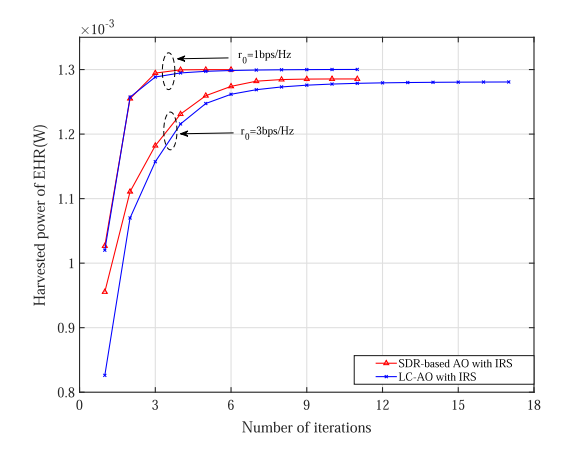
\includegraphics[width=9cm]{fig2.png}
    \caption{Fig. 2. Harvested power of EHR versus the number of iterations.}
    \label{Fig. 1.}
\end{figure}
\end{frame}
\begin{frame}{Simulation results}
    \begin{figure}[htp]
    \centering
    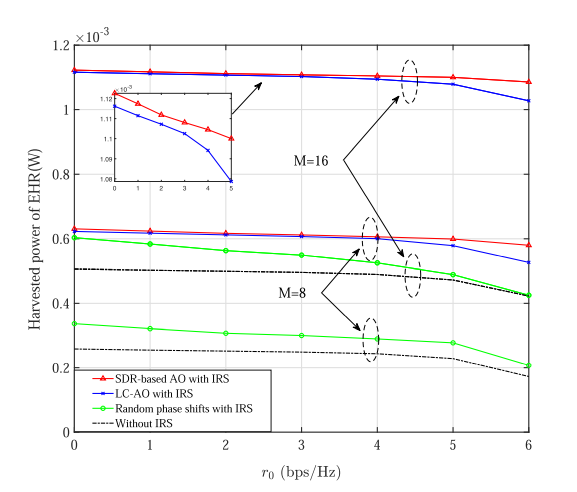
\includegraphics[width=9cm]{fig3.png}
    \caption{Fig. 3. Harvested power of EHR versus $r_{0}$}
    \label{Fig. 1.}
\end{figure}
\end{frame}
\begin{frame}
    \begin{figure}[htp]
    \centering
    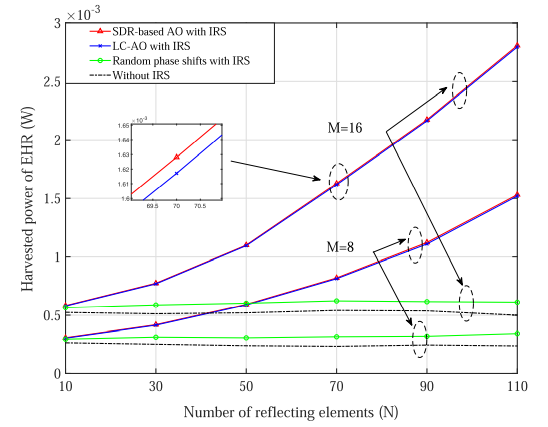
\includegraphics[width=9cm]{fig4.png}
    \caption{Fig. 4.  Harvested power of EHR versus N}
    \label{Fig. 1.}
\end{figure}
\end{frame}
\begin{frame}{Conclusion}
    \begin{enumerate}
        \item Two alternating iterative algorithms
SDR and LC-AO were proposed to address the non-convex
optimization problem.
\item With a much lower-complexity, the proposed LC-AO method can achieve almost the same
performance as the proposed SDR method
\item the proposed two methods approximately double the harvested power compared to existing methods.
    \end{enumerate}
\end{frame}

\end{document}